\documentclass[11pt,a4paper,landscape]{article}
\usepackage[margin=10mm]{geometry}
\usepackage{graphicx}
\usepackage{tikz}
\usetikzlibrary{arrows.meta,positioning,fit,backgrounds,shapes.geometric}
\usepackage{array}
\usepackage{xcolor}
\pagestyle{empty}

\definecolor{inputblue}{RGB}{222,238,255}
\definecolor{processgreen}{RGB}{225,244,232}
\definecolor{branchyellow}{RGB}{255,245,210}
\definecolor{outputred}{RGB}{255,230,230}
\definecolor{notegrey}{RGB}{244,244,244}
\definecolor{titlegreen}{RGB}{0,42,28}
\definecolor{stageblue}{RGB}{52,177,235}
\definecolor{flowgreen}{RGB}{183,239,205}
\definecolor{datagreen}{RGB}{16,190,95}
\definecolor{metapurple}{RGB}{226,143,238}
\definecolor{calibyellow}{RGB}{255,225,88}
\definecolor{framegreen}{RGB}{36,174,95}
\definecolor{linegreen}{RGB}{19,83,62}
\definecolor{depred}{RGB}{245,135,135}

\tikzset{
  box/.style={
    draw,
    rounded corners=2pt,
    align=center,
    minimum height=9mm,
    text width=34mm,
    font=\scriptsize,
    inner sep=3pt
  },
  widebox/.style={
    box,
    text width=48mm
  },
  smallbox/.style={
    box,
    text width=28mm
  },
  input/.style={box, fill=inputblue},
  process/.style={box, fill=processgreen},
  branch/.style={box, fill=branchyellow},
  output/.style={box, fill=outputred},
  note/.style={box, fill=notegrey},
  arrow/.style={-{Latex[length=2.1mm]}, thick},
  lightarrow/.style={-{Latex[length=1.8mm]}, thin},
  fcframe/.style={draw=framegreen, rounded corners=2pt, line width=0.55pt},
  fctitle/.style={fill=titlegreen, text=white, font=\bfseries\large, align=center, inner sep=4pt},
  fcstage/.style={fill=stageblue, text=black, font=\bfseries\normalsize, align=center, inner sep=3pt},
  fcop/.style={draw=none, fill=flowgreen, align=center, font=\scriptsize, text width=25mm, minimum height=8mm, inner sep=2pt},
  fcopwide/.style={fcop, text width=32mm},
  fcdata/.style={draw=none, fill=datagreen, ellipse, align=center, font=\scriptsize, text width=22mm, minimum height=9mm, inner sep=1.5pt},
  fcmeta/.style={draw=none, fill=metapurple, align=center, font=\scriptsize, text width=23mm, minimum height=8mm, inner sep=2pt},
  fcfeature/.style={draw=none, fill=metapurple, diamond, aspect=1.8, align=center, font=\scriptsize, text width=16mm, inner sep=0.8pt},
  fccalib/.style={draw=none, fill=calibyellow, align=center, font=\scriptsize, text width=22mm, minimum height=29mm, inner sep=2pt},
  fcsmallnote/.style={align=center, font=\tiny, text width=25mm, inner sep=1pt},
  fcarrow/.style={-{Latex[length=1.7mm]}, draw=linegreen, line width=0.55pt},
  fcdep/.style={-{Latex[length=1.5mm]}, draw=depred, line width=0.35pt, dotted},
}

\begin{document}

\noindent\resizebox{0.985\linewidth}{!}{%
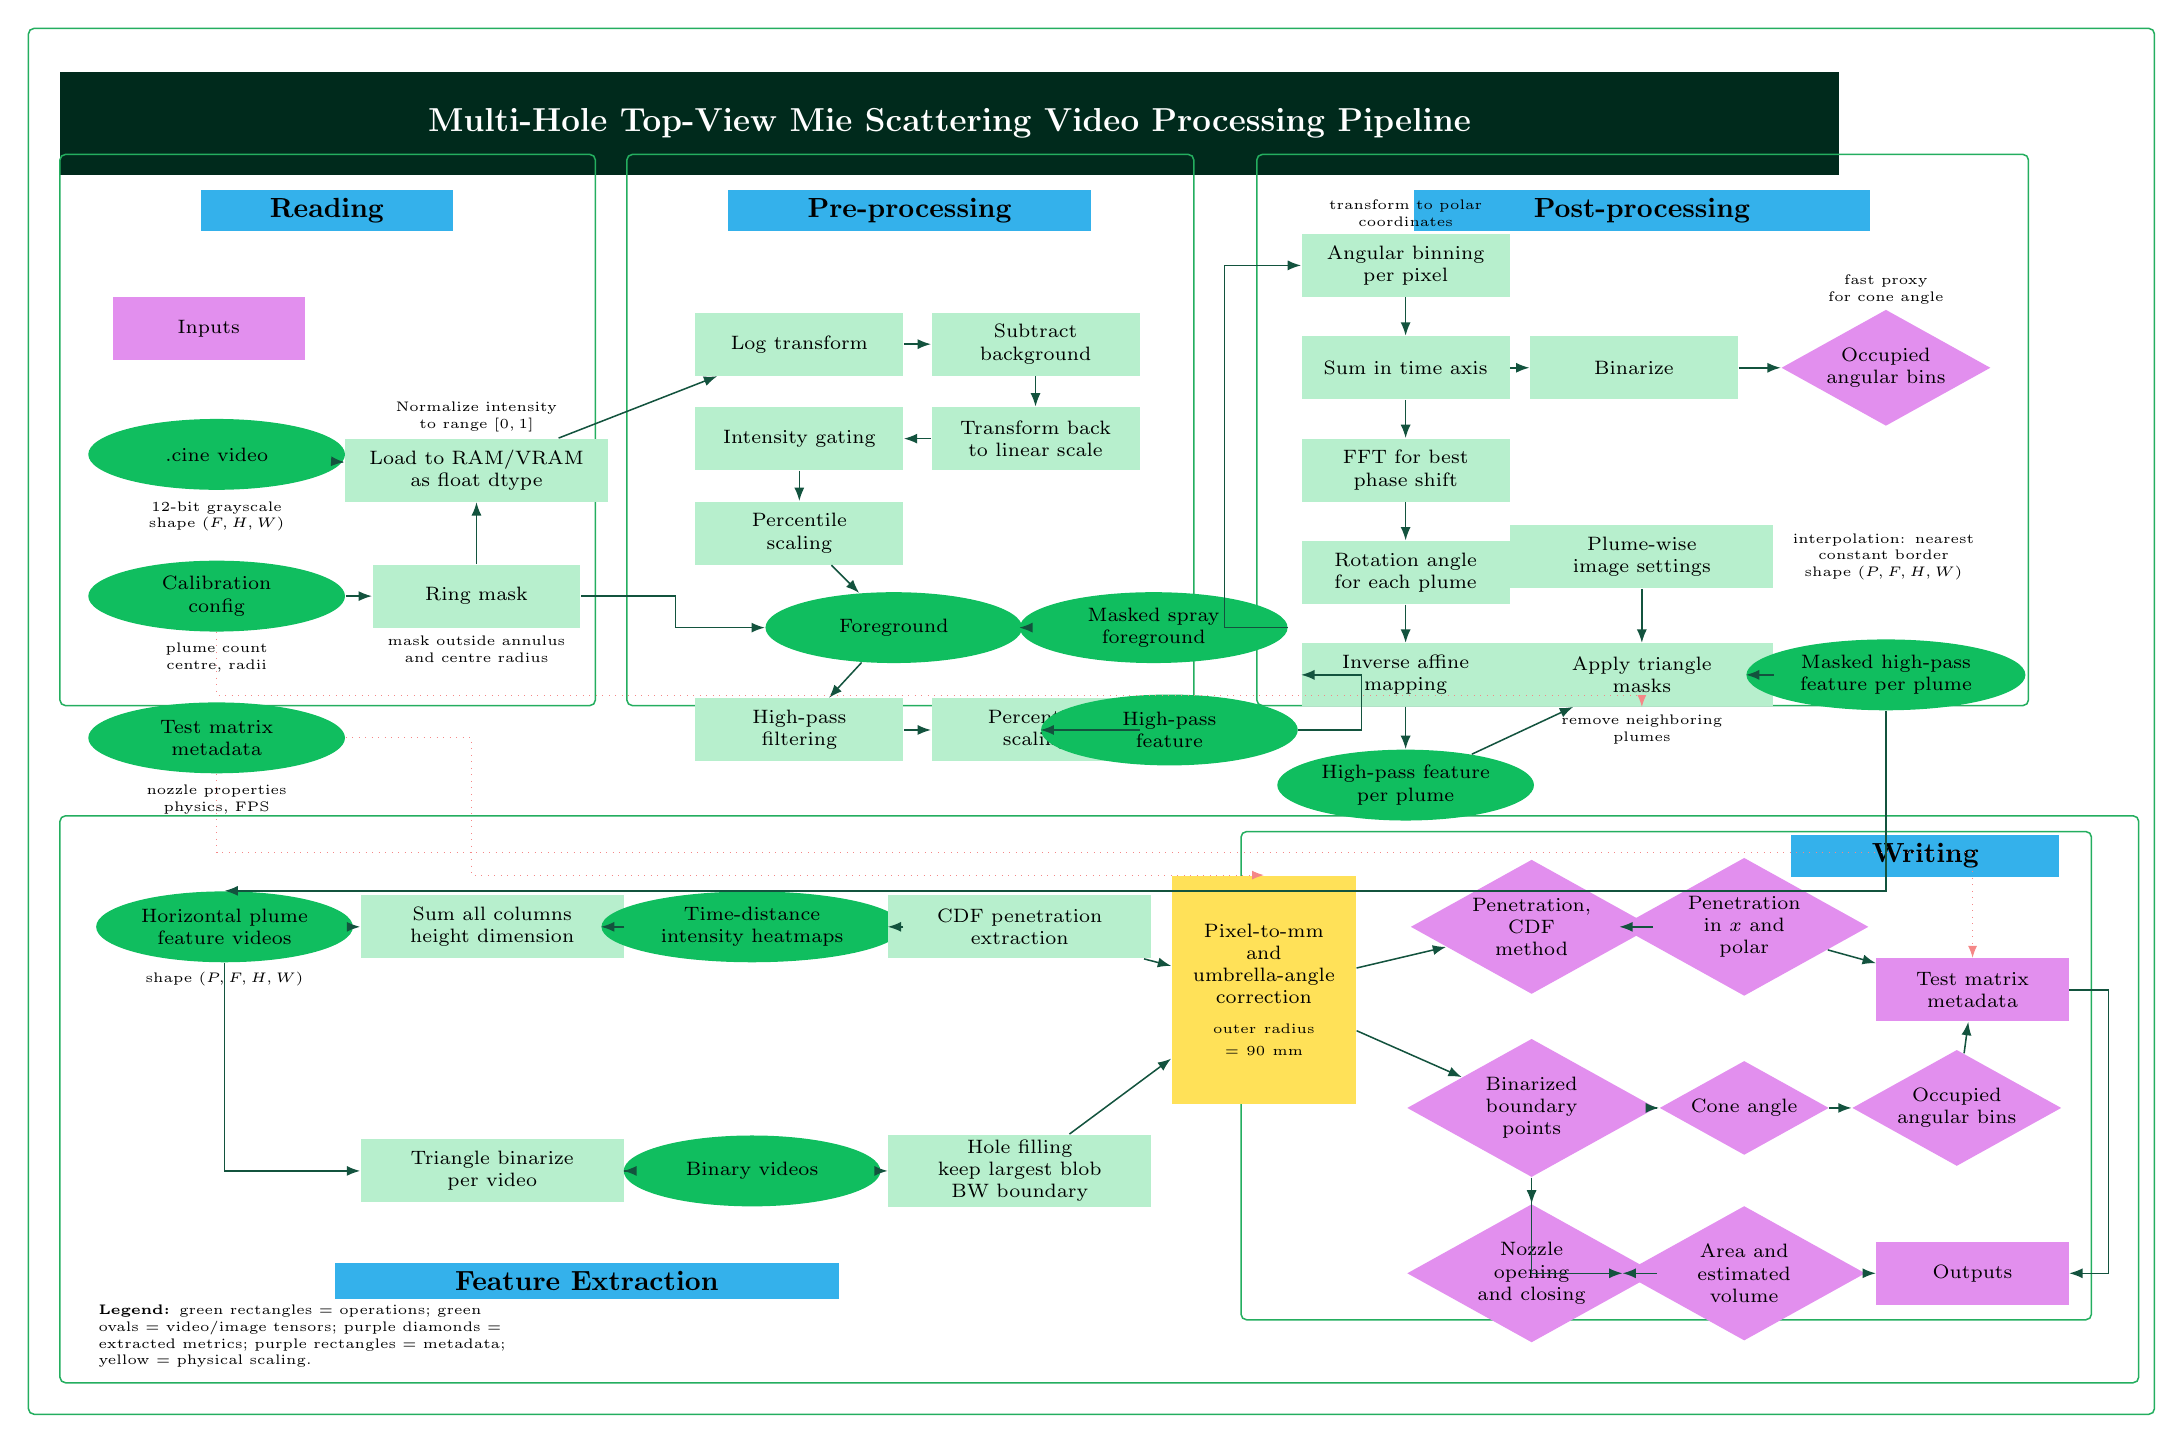
\begin{tikzpicture}[x=1mm,y=1mm]

% Canvas and title
\node[fcframe, minimum width=270mm, minimum height=176mm, anchor=south west] at (6,4) {};
\node[fctitle, minimum width=226mm, minimum height=13mm, anchor=west] at (10,168)
  {Multi-Hole Top-View Mie Scattering Video Processing Pipeline};

% Stage frames
\node[fcframe, minimum width=68mm, minimum height=70mm, anchor=south west] at (10,94) {};
\node[fcstage, minimum width=32mm] at (44,157) {Reading};

\node[fcframe, minimum width=72mm, minimum height=70mm, anchor=south west] at (82,94) {};
\node[fcstage, minimum width=46mm] at (118,157) {Pre-processing};

\node[fcframe, minimum width=98mm, minimum height=70mm, anchor=south west] at (162,94) {};
\node[fcstage, minimum width=58mm] at (211,157) {Post-processing};

\node[fcframe, minimum width=264mm, minimum height=72mm, anchor=south west] at (10,8) {};
\node[fcframe, minimum width=108mm, minimum height=62mm, anchor=south west] at (160,16) {};
\node[fcstage, minimum width=64mm] at (77,21) {Feature Extraction};
\node[fcstage, minimum width=34mm] at (247,75) {Writing};

% Reading
\node[fcmeta, minimum width=23mm] (inputs) at (29,142) {Inputs};
\node[fcdata] (cine) at (30,126) {.cine video};
\node[fcsmallnote, below=1mm of cine] {12-bit grayscale\\shape $(F,H,W)$};
\node[fcdata] (cfg) at (30,108) {Calibration\\config};
\node[fcsmallnote, below=1mm of cfg] {plume count\\centre, radii};
\node[fcdata] (tm) at (30,90) {Test matrix\\metadata};
\node[fcsmallnote, below=1mm of tm] {nozzle properties\\physics, FPS};
\node[fcopwide] (load) at (63,124) {Load to RAM/VRAM\\as float dtype};
\node[fcsmallnote, above=0.4mm of load] {Normalize intensity\\to range $[0,1]$};
\node[fcop] (ring) at (63,108) {Ring mask};
\node[fcsmallnote, below=0.6mm of ring] {mask outside annulus\\and centre radius};
\draw[fcarrow] (cine) -- (load);
\draw[fcarrow] (cfg) -- (ring);
\draw[fcarrow] (ring) -- (load);

% Pre-processing
\node[fcop] (logt) at (104,140) {Log transform};
\node[fcop] (subbg) at (134,140) {Subtract\\background};
\node[fcop] (linear) at (134,128) {Transform back\\to linear scale};
\node[fcop] (gate) at (104,128) {Intensity gating};
\node[fcop] (pscale1) at (104,116) {Percentile\\scaling};
\node[fcdata] (fg) at (116,104) {Foreground};
\node[fcop] (hpfilter) at (104,91) {High-pass\\filtering};
\node[fcop] (pscale2) at (134,91) {Percentile\\scaling};
\node[fcdata] (hpfeat) at (151,91) {High-pass\\feature};
\node[fcdata, text width=23mm] (maskedfg) at (149,104) {Masked spray\\foreground};
\draw[fcarrow] (load) -- (logt);
\draw[fcarrow] (logt) -- (subbg);
\draw[fcarrow] (subbg) -- (linear);
\draw[fcarrow] (linear) -- (gate);
\draw[fcarrow] (gate) -- (pscale1);
\draw[fcarrow] (pscale1) -- (fg);
\draw[fcarrow] (ring.east) -- ++(12,0) |- (fg.west);
\draw[fcarrow] (fg) -- (maskedfg);
\draw[fcarrow] (fg) -- (hpfilter);
\draw[fcarrow] (hpfilter) -- (pscale2);
\draw[fcarrow] (pscale2) -- (hpfeat);

% Post-processing
\node[fcop] (angbin) at (181,150) {Angular binning\\per pixel};
\node[fcsmallnote, above=0.5mm of angbin] {transform to polar\\coordinates};
\node[fcop] (sumt) at (181,137) {Sum in time axis};
\node[fcop] (fft) at (181,124) {FFT for best\\phase shift};
\node[fcop] (rotang) at (181,111) {Rotation angle\\for each plume};
\node[fcop] (affine) at (181,98) {Inverse affine\\mapping};
\node[fcdata, text width=22mm] (plumehp) at (181,84) {High-pass feature\\per plume};
\node[fcop] (binz) at (210,137) {Binarize};
\node[fcfeature] (occ1) at (242,137) {Occupied\\angular bins};
\node[fcopwide] (settings) at (211,113) {Plume-wise\\image settings};
\node[fcsmallnote, right=1mm of settings] {interpolation: nearest\\constant border\\shape $(P,F,H,W)$};
\node[fcopwide] (triangles) at (211,98) {Apply triangle\\masks};
\node[fcsmallnote, below=0.6mm of triangles] {remove neighboring\\plumes};
\node[fcdata, text width=24mm] (maskedhp) at (242,98) {Masked high-pass\\feature per plume};
\node[fcsmallnote, above=0.2mm of occ1] {fast proxy\\for cone angle};
\draw[fcarrow] (maskedfg) -- ++(9,0) |- (angbin.west);
\draw[fcarrow] (angbin) -- (sumt);
\draw[fcarrow] (sumt) -- (binz);
\draw[fcarrow] (binz) -- (occ1);
\draw[fcarrow] (sumt) -- (fft);
\draw[fcarrow] (fft) -- (rotang);
\draw[fcarrow] (rotang) -- (affine);
\draw[fcarrow] (hpfeat.east) -- ++(8,0) |- (affine.west);
\draw[fcarrow] (affine) -- (plumehp);
\draw[fcarrow] (settings) -- (triangles);
\draw[fcarrow] (plumehp) -- (triangles);
\draw[fcarrow] (triangles) -- (maskedhp);

% Feature extraction, CDF branch
\node[fcdata] (hvid) at (31,66) {Horizontal plume\\feature videos};
\node[fcsmallnote, below=0.8mm of hvid] {shape $(P,F,H,W)$};
\node[fcopwide] (sumcols) at (65,66) {Sum all columns\\height dimension};
\node[fcdata, text width=26mm] (heatmap) at (98,66) {Time-distance\\intensity heatmaps};
\node[fcopwide] (cdfext) at (132,66) {CDF penetration\\extraction};
\node[fccalib] (correction) at (163,58) {Pixel-to-mm\\and\\umbrella-angle\\correction\\[1mm]\tiny outer radius = 90 mm};
\node[fcfeature] (cdfmethod) at (197,66) {Penetration,\\CDF method};
\node[fcfeature] (penetration) at (224,66) {Penetration\\in $x$ and polar};
\draw[fcarrow] (maskedhp.south) |- (hvid.north);
\draw[fcarrow] (hvid) -- (sumcols);
\draw[fcarrow] (sumcols) -- (heatmap);
\draw[fcarrow] (heatmap) -- (cdfext);
\draw[fcarrow] (cdfext) -- (correction);
\draw[fcarrow] (correction) -- (cdfmethod);
\draw[fcarrow] (cdfmethod) -- (penetration);

% Feature extraction, binary boundary branch
\node[fcopwide] (tribin) at (65,35) {Triangle binarize\\per video};
\node[fcdata] (bwvid) at (98,35) {Binary videos};
\node[fcopwide] (holefill) at (132,35) {Hole filling\\keep largest blob\\BW boundary};
\node[fcfeature] (boundary) at (197,43) {Binarized\\boundary points};
\node[fcfeature] (cone) at (224,43) {Cone angle};
\node[fcfeature] (occ2) at (251,43) {Occupied\\angular bins};
\node[fcfeature] (area) at (224,22) {Area and\\estimated volume};
\node[fcfeature] (openclose) at (197,22) {Nozzle opening\\and closing};
\draw[fcarrow] (hvid.south) |- (tribin.west);
\draw[fcarrow] (tribin) -- (bwvid);
\draw[fcarrow] (bwvid) -- (holefill);
\draw[fcarrow] (holefill) -- (correction);
\draw[fcarrow] (correction) -- (boundary);
\draw[fcarrow] (boundary) -- (cone);
\draw[fcarrow] (cone) -- (occ2);
\draw[fcarrow] (boundary) |- (area);
\draw[fcarrow] (boundary.south) -- (openclose.north);

% Metadata dependencies and output
\node[fcmeta, minimum width=20mm] (outmeta) at (253,58) {Test matrix\\metadata};
\node[fcmeta, minimum width=20mm] (outputs) at (253,22) {Outputs};
\draw[fcarrow] (penetration) -- (outmeta);
\draw[fcarrow] (occ2) -- (outmeta);
\draw[fcarrow] (outmeta.east) -- ++(5,0) |- (outputs.east);
\draw[fcarrow] (openclose.east) -- (area.west);
\draw[fcarrow] (area.east) -- (outputs.west);
\draw[fcdep] (tm.east) -- ++(16,0) |- (correction.north);
\draw[fcdep] (cfg.south) -- ++(0,-8) -| (triangles.south);
\draw[fcdep] (tm.south) -- ++(0,-10) -| (outmeta.north);

% Compact legend
\node[fcsmallnote, align=left, text width=54mm] at (42,14)
  {\textbf{Legend:} green rectangles = operations; green ovals = video/image tensors; purple diamonds = extracted metrics; purple rectangles = metadata; yellow = physical scaling.};

\end{tikzpicture}%
}

\vfill
\scriptsize
Code anchors: \texttt{mie\_multi\_hole.py:\_process\_cine\_file}, \texttt{OSCC\_postprocessing.analysis.mie\_multihole}, and \texttt{OSCC\_postprocessing.binary\_ops.feature\_extraction}. The first page follows the detailed visual prototype: it separates reading, preprocessing, polar/plume-wise postprocessing, feature extraction, and final tabular outputs while keeping metadata/config dependencies as dotted red links.

\newpage

\begin{center}
\Large\bfseries Fit Raw Data Pipeline: 1D Metrics to Curve Parameters
\end{center}

\vspace{-1mm}

\noindent\resizebox{0.98\linewidth}{!}{%
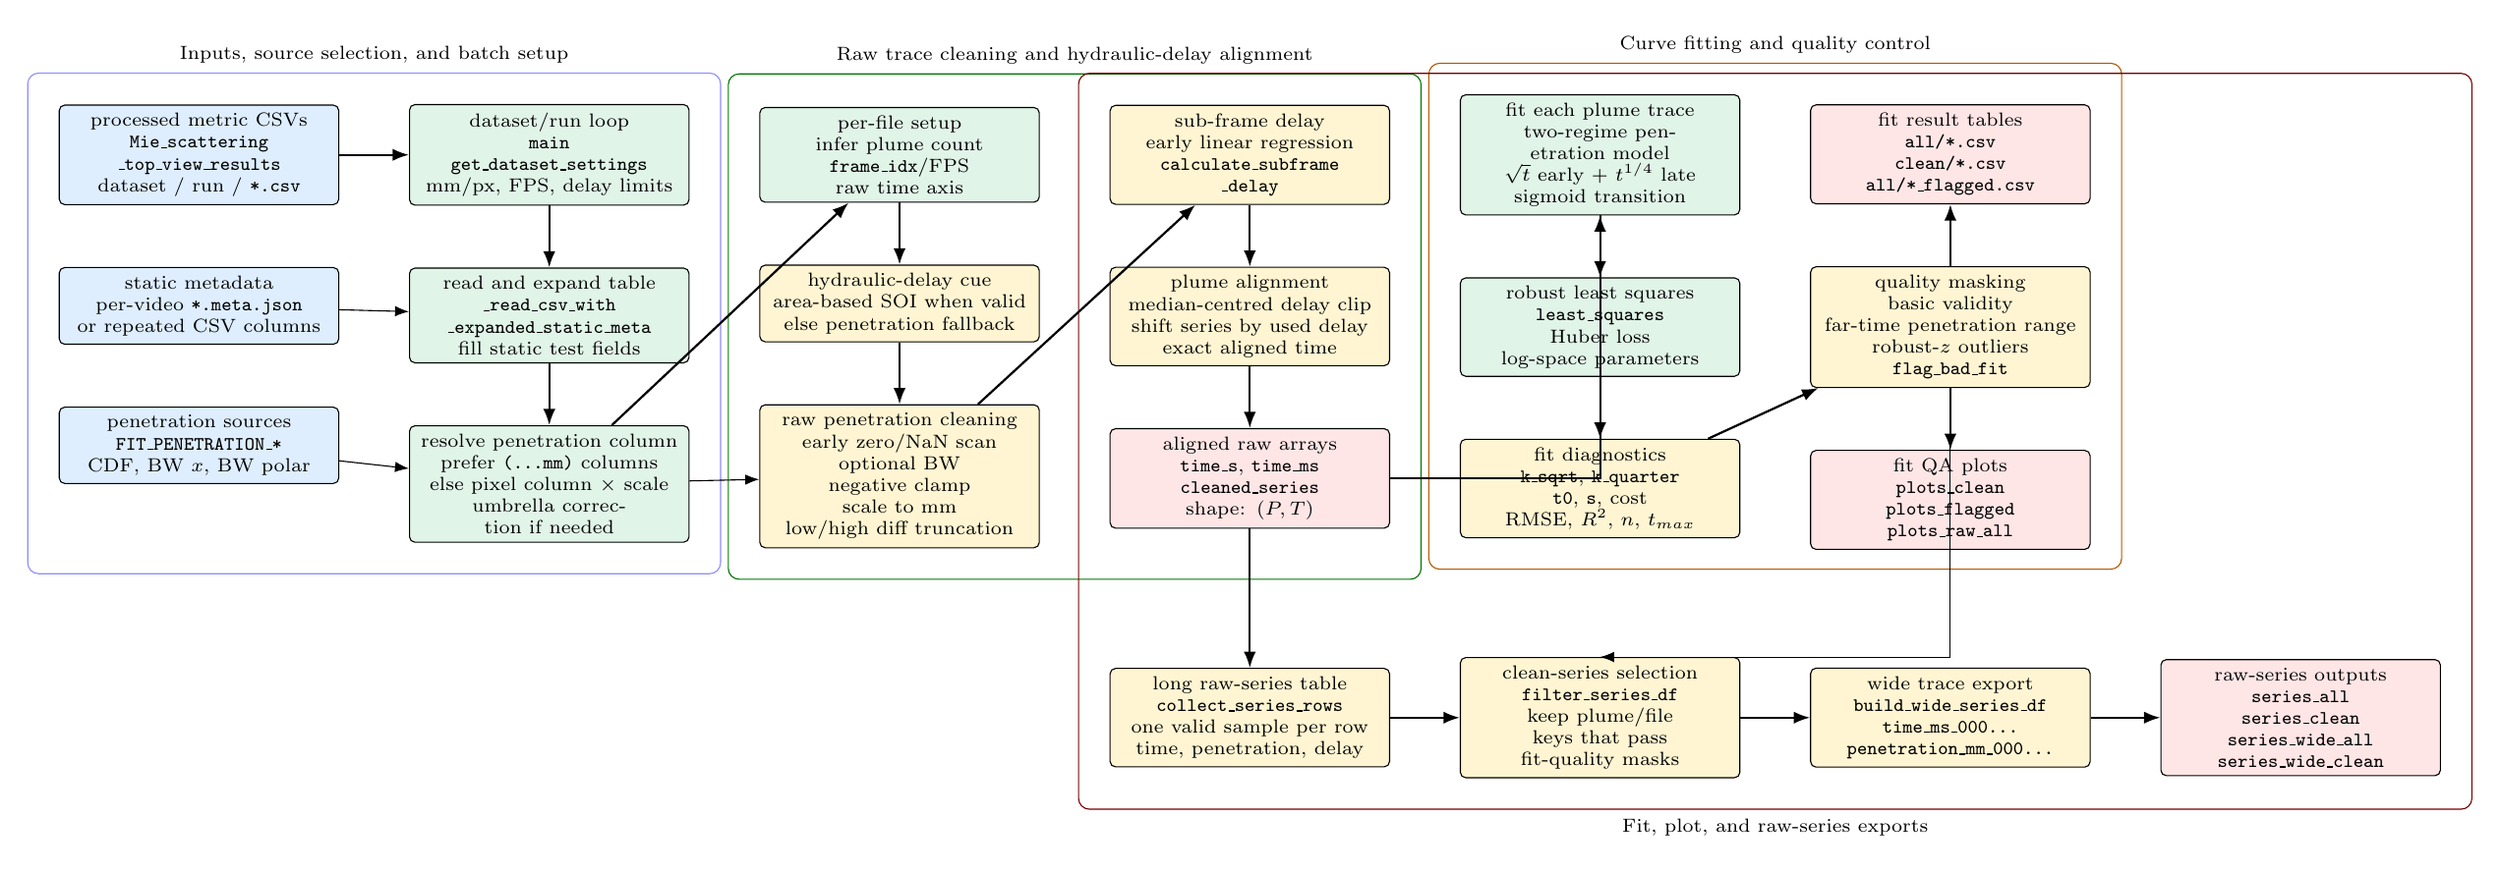
\begin{tikzpicture}[node distance=8mm and 9mm]

% Inputs and batch setup
\node[input] (csvs) {processed metric CSVs\\\texttt{Mie\_scattering}\\\texttt{\_top\_view\_results}\\dataset / run / \texttt{*.csv}};
\node[input, below=of csvs] (metajson) {static metadata\\per-video \texttt{*.meta.json}\\or repeated CSV columns};
\node[input, below=of metajson] (sources) {penetration sources\\\texttt{FIT\_PENETRATION\_*}\\CDF, BW $x$, BW polar};

\node[process, right=of csvs] (loop) {dataset/run loop\\\texttt{main}\\\texttt{get\_dataset\_settings}\\mm/px, FPS, delay limits};
\node[process, below=of loop] (read) {read and expand table\\\texttt{\_read\_csv\_with}\\\texttt{\_expanded\_static\_meta}\\fill static test fields};
\node[process, below=of read] (resolve) {resolve penetration column\\prefer \texttt{(...mm)} columns\\else pixel column $\times$ scale\\umbrella correction if needed};

\draw[arrow] (csvs) -- (loop);
\draw[arrow] (loop) -- (read);
\draw[lightarrow] (metajson) -- (read);
\draw[lightarrow] (sources) -- (resolve);
\draw[arrow] (read) -- (resolve);

% Per-file series preparation
\node[process, right=of loop] (axes) {per-file setup\\infer plume count\\\texttt{frame\_idx}/FPS\\raw time axis};
\node[branch, below=of axes] (delay) {hydraulic-delay cue\\area-based SOI when valid\\else penetration fallback};
\node[branch, below=of delay] (clean) {raw penetration cleaning\\early zero/NaN scan\\optional BW negative clamp\\scale to mm\\low/high diff truncation};

\draw[arrow] (resolve) -- (axes);
\draw[arrow] (axes) -- (delay);
\draw[arrow] (delay) -- (clean);
\draw[lightarrow] (resolve) -- (clean);

% Delay refinement and aligned arrays
\node[branch, right=of axes] (subdelay) {sub-frame delay\\early linear regression\\\texttt{calculate\_subframe}\\\texttt{\_delay}};
\node[branch, below=of subdelay] (align) {plume alignment\\median-centred delay clip\\shift series by used delay\\exact aligned time};
\node[output, below=of align] (aligned) {aligned raw arrays\\\texttt{time\_s}, \texttt{time\_ms}\\\texttt{cleaned\_series}\\shape: $(P,T)$};

\draw[arrow] (clean) -- (subdelay);
\draw[arrow] (subdelay) -- (align);
\draw[arrow] (align) -- (aligned);

% Fit branch
\node[process, right=of subdelay] (fitmodel) {fit each plume trace\\two-regime penetration model\\$\sqrt{t}$ early + $t^{1/4}$ late\\sigmoid transition};
\node[process, below=of fitmodel] (solver) {robust least squares\\\texttt{least\_squares}\\Huber loss\\log-space parameters};
\node[branch, below=of solver] (diagnostics) {fit diagnostics\\\texttt{k\_sqrt}, \texttt{k\_quarter}\\\texttt{t0}, \texttt{s}, cost\\RMSE, $R^2$, $n$, $t_{max}$};

\draw[arrow] (aligned) -| (fitmodel);
\draw[arrow] (fitmodel) -- (solver);
\draw[arrow] (solver) -- (diagnostics);

% Quality masking and fit outputs
\node[branch, right=of solver] (mask) {quality masking\\basic validity\\far-time penetration range\\robust-$z$ outliers\\\texttt{flag\_bad\_fit}};
\node[output, above=of mask] (fitcsv) {fit result tables\\\texttt{all/*.csv}\\\texttt{clean/*.csv}\\\texttt{all/*\_flagged.csv}};
\node[output, below=of mask] (plots) {fit QA plots\\\texttt{plots\_clean}\\\texttt{plots\_flagged}\\\texttt{plots\_raw\_all}};

\draw[arrow] (diagnostics) -- (mask);
\draw[arrow] (mask) -- (fitcsv);
\draw[arrow] (mask) -- (plots);

% Raw-series export branch
\node[branch, below=18mm of aligned] (seriesrows) {long raw-series table\\\texttt{collect\_series\_rows}\\one valid sample per row\\time, penetration, delay};
\node[branch, right=of seriesrows] (seriesclean) {clean-series selection\\\texttt{filter\_series\_df}\\keep plume/file keys that pass\\fit-quality masks};
\node[branch, right=of seriesclean] (wide) {wide trace export\\\texttt{build\_wide\_series\_df}\\\texttt{time\_ms\_000...}\\\texttt{penetration\_mm\_000...}};
\node[output, right=of wide] (seriesout) {raw-series outputs\\\texttt{series\_all}\\\texttt{series\_clean}\\\texttt{series\_wide\_all}\\\texttt{series\_wide\_clean}};

\draw[arrow] (aligned) -- (seriesrows);
\draw[arrow] (seriesrows) -- (seriesclean);
\draw[arrow] (seriesclean) -- (wide);
\draw[arrow] (wide) -- (seriesout);
\draw[lightarrow] (mask.south) |- (seriesclean.north);

% Grouping backgrounds
\begin{scope}[on background layer]
  \node[draw=blue!45, rounded corners=4pt, fit=(csvs)(metajson)(sources)(loop)(read)(resolve), inner sep=4mm, label={[font=\scriptsize]above:Inputs, source selection, and batch setup}] {};
  \node[draw=green!45!black, rounded corners=4pt, fit=(axes)(delay)(clean)(subdelay)(align)(aligned), inner sep=4mm, label={[font=\scriptsize]above:Raw trace cleaning and hydraulic-delay alignment}] {};
  \node[draw=orange!70!black, rounded corners=4pt, fit=(fitmodel)(solver)(diagnostics)(mask), inner sep=4mm, label={[font=\scriptsize]above:Curve fitting and quality control}] {};
  \node[draw=red!45!black, rounded corners=4pt, fit=(fitcsv)(plots)(seriesrows)(seriesclean)(wide)(seriesout), inner sep=4mm, label={[font=\scriptsize]below:Fit, plot, and raw-series exports}] {};
\end{scope}

\end{tikzpicture}%
}

\vfill
\scriptsize
Code anchors: \texttt{MLP/fit\_raw\_data.py:main}, \texttt{process\_folder}, \texttt{prepare\_cleaned\_series}, \texttt{fit\_sigmoid}, \texttt{apply\_filter\_masking}, \texttt{build\_wide\_series\_df}, and \texttt{save\_fit\_plot}. The diagram shows the per-penetration-source path from processed 1D plume metrics to fitted curve parameters, quality flags, QA plots, and raw-series exports.

\end{document}
